
\chapter{Fuerzas centrales}

\section{Problema de dos cuerpos}
El problema de la interacción de dos cuerpos bajo el efecto de una fuerza central se puede solucionar analíticamente, transformando el problema de dos cuerpos a un problema equivalente de un sólo cuerpo. Desafortunadamente el método no puede ser generalizado. No hay forma de reducir el problema de tres o más partículas a uno equivalente de un sólo cuerpo, por está razón la solución del problema de tres cuerpos sólo puede hacerse numéricamente. 

Considere un sistema aislado que conste de dos partículas interactuando bajo una fuerza central $\mathbf{F}(\mathbf{r})$, como se ilustra en la figura~\ref{fig:fuerzascentrales}
\begin{figure}
  \centering
  \includegraphics{fuerzascentrales}
  \caption{Fuerzas centrales atractivas}
  \label{fig:fuerzascentrales}
\end{figure}

De la tercera ley de Newton tenemos que la fuerza que ejerce la partícula 2 sobre la partícula 1 es
\begin{align}
  \mathbf{F}=\mathbf{F}_{12}=-\mathbf{F}_{21}=F(r)\hat{\mathbf{r}}\,,
\end{align}
donde $\mathbf{F}_{21}$ es la fuerza de reacción que ejerce la partícula 1 sobre la 2 y
\begin{align}
  \label{eq:rcentral}
  \mathbf{r}=\mathbf{r}_1-\mathbf{r}_2\,.
\end{align}

Las ecuaciones de movimiento son
\begin{align}
  \label{eq:edmfc}
  m_1\ddot{\mathbf{r}}_1=&\mathbf{F}_{12}=\mathbf{F}=F(r)\hat{\mathbf{r}}\nonumber\\
  m_2\ddot{\mathbf{r}}_2=&\mathbf{F}_{21}=-\mathbf{F}=-F(r)\hat{\mathbf{r}}\,.
\end{align}

De las convenciones en la figura~\ref{fig:fuerzascentrales} para el caso de fuerzas atractivas podemos observar que la dirección de $\mathbf{F}_{12}$ es opuesta al vector unitario $\hat{\mathbf{r}}$, por lo tanto $F(r)<0$. El caso $F(r)>0$ corresponde a un par de fuerzas atractivas. 

El problema se simplifica si reemplazamos las coordenadas $\mathbf{r}_1$ y $\mathbf{r}_2$ por $\mathbf{r}$ y el vector de centro de masa $\mathbf{R}$, donde
\begin{align}
  \label{eq:Rcm}
  \mathbf{R}=&\frac{m_1\mathbf{r}_1+m_2\mathbf{r}_2}{m_1+m_2}\nonumber\\
  M=&m_1+m_2\,.
\end{align}
La ecuación de movimiento para $\mathbf{R}$ es
\begin{align}
  M \ddot{\mathbf{R}}=&\frac{M}{M}(m_1\ddot{\mathbf{r}}_1+m_2\ddot{\mathbf{r}}_2)\nonumber\\
  =&\mathbf{F}_{12}+\mathbf{F}_{21}\nonumber\\
  =&\mathbf{F}_{12}-\mathbf{F}_{12}\nonumber\\
  =&0\,.
\end{align}
Sobre la partícula equivalente de masa $M$ y en la posición del centro de masa $\mathbf{R}$ no tiene fuerzas externas actuando sobre ellas y por tanto se mueve a velocidad $\mathbf{V}=\dot{\mathbf{R}}$ constante, con ecuación de movimiento
\begin{align}
  \mathbf{R}=\mathbf{R}_0+\mathbf{V}t\,.
\end{align}
Las constantes $\mathbf{R}_0$ y $\mathbf{V}$ dependen de la escogencia del sistema de referencia y de las condiciones iniciales. 

Para encontrar las ecuaciones de movimiento para $\mathbf{r}$ usaremos la ec.~\eqref{eq:edmfc}
\begin{align}
  \ddot{\mathbf{r}}_1=&\frac{F(r)}{m_1}\hat{\mathbf{r}}\nonumber\\
  \ddot{\mathbf{r}}_2=&-\frac{F(r)}{m_2}\hat{\mathbf{r}}\,.
\end{align}
que al restarlas dan lugar a
\begin{align}
  \label{eq:prevcentral}
  \ddot{\mathbf{r}}_1-\ddot{\mathbf{r}}_2=&\left(\frac{1}{m_1}+\frac{1}{m_2}\right)F(r)\hat{\mathbf{r}}\nonumber\\
  =&\frac{m_1 m_2}{m_1+m_2}F(r)\hat{\mathbf{r}}\nonumber\\
  =&\mu F(r)\hat{\mathbf{r}}\,,
\end{align}
donde hemos definido la masa reducida
\begin{align}
  \mu=  \frac{m_1 m_2}{m_1+m_2}\,.
\end{align}
Además, derivando dos veces la ec.~\eqref{eq:rcentral}
\begin{align}
   \ddot{\mathbf{r}}=\ddot{\mathbf{r}}_1-\ddot{\mathbf{r}}_2\,,
\end{align}
podemos escribir la ec.~\eqref{eq:prevcentral} como una ecuación de movimiento para una partícula de masa $\mu$ bajo el efecto de una fuerza $F(r)\hat{\mathbf{r}}$ como
\begin{align}
  \label{eq:singlebody}
  \ddot{\mathbf{r}}=\mu F(r)\hat{\mathbf{r}}\,.
\end{align}
y el problema de dos cuerpos se reduce al problema de una sola partícula como se ilustra en la figura~\ref{fig:singlecentral}
\begin{figure}
  \centering
  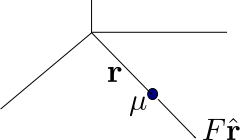
\includegraphics{singlecentral}
  \caption{Reducción del problema de dos cuerpos al problema de un sólo cuerpo}
  \label{fig:singlecentral}
\end{figure}
El problema ahora es encontrar $\mathbf{r}$ como una función del tiempo a partir de la ec.~\eqref{eq:singlebody}, pero esto no es posible sin antes especificar $F(r)$. Suponiendo que podemos encontrar $\mathbf{r}$, podemos encontrar $\mathbf{r}_1$ y $\mathbf{r}_2$, usando las relaciones \eqref{eq:rcentral} y \eqref{eq:Rcm}, solucionando para $\mathbf{r}_1$ y $\mathbf{r}_2$. De \eqref{eq:Rcm}
\begin{align}
  (m_1+m_2)\mathbf{R}=&m_1\mathbf{r}_1+m_2\mathbf{r}_2\,,
\end{align}
y usando \eqref{eq:rcentral}
\begin{align}
   (m_1+m_2)\mathbf{R}=&m_1(\mathbf{r}+\mathbf{r}_2)+m_2\mathbf{r}_2\nonumber\\
     (m_1+m_2)\mathbf{R}=&m_1\mathbf{r}+m_1\mathbf{r}_2+m_2\mathbf{r}_2\nonumber\\
     (m_1+m_2)\mathbf{R}=&m_1\mathbf{r}+\mathbf{r}_2(m_1+m_2)\,,
\end{align}
despejando $\mathbf{R}$
\begin{align}
     \mathbf{R}=&\frac{m_1}{m_1+m_2}\mathbf{r}+\mathbf{r}_2\,,
\end{align}
obtenemos
\begin{align}
\label{eq:r2}
  \mathbf{r}_2=\mathbf{R}-\frac{m_1}{m_1+m_2}\mathbf{r}\,,
\end{align}
y usando de nuevo \eqref{eq:rcentral}
\begin{align}
\label{eq:r1}
  \mathbf{r}_1=&\mathbf{r}+\mathbf{r_2}\nonumber\\
  =&\mathbf{r}+\mathbf{R}-\frac{m_1}{m_1+m_2}\mathbf{r}\nonumber\\
  =&\mathbf{R}+\left(1-\frac{m_1}{m_1+m_2}\right)\mathbf{r}\nonumber\\
  =&\mathbf{R}+\frac{m_1+m_2-m_1}{m_1+m_2}\mathbf{r}\nonumber\\
  \mathbf{r}_1  =&\mathbf{R}+\frac{m_2}{m_1+m_2}\mathbf{r}\,.
\end{align}

\section{Propiedades generales del movimiento bajo fuerzas centrales}
Antes de abordar soluciones específicas establezcamos las propiedades generales del movimiento bajo fuerzas centrales
\begin{align}
  \label{eq:singlebody2}
  F(r)\hat{\mathbf{r}}=\mu \ddot{\mathbf{r}}\,.
\end{align}
Aunque formalmente la ecuación \eqref{eq:singlebody2} corresponde a un sistema de tres ecuaciones, con la ayuda de las leyes de conservación se puede reducir a una sola ecuación.

\subsection{El movimiento está confinado a un plano}
Lo cual reduce el problema a uno de dos ecuaciones. Para demostrar esta propiedad del movimiento bajo fuerzas centrales, partimos del hecho que la fuerza $F(r)\hat{\mathbf{r}}$, es a lo largo de $\hat{\mathbf{r}}$ y por consiguiente no puede ejercer torque sobre la masa reducida $\mu$, es decir
\begin{align}
  \mathbf{r}\times\mathbf{F}=F(r)\mathbf{r}\times\hat{\mathbf{r}}=0\,,
\end{align}
En ausencia de torques externos entonces el moméntum angular se debe conservar. Ya que
\begin{align}
  \mathbf{L}=\mathbf{r}\times \mu \mathbf{v}\,,
\end{align}
donde $\mathbf{v}=\dot{\mathbf{r}}$, entonces $\mathbf{r}$ debe ser perpendicular a $\mathbf{L}$. Ya que $\mathbf{L}$ está fijo en el espacio $\mathbf{r}$ tiene que permanecer en el plano perpendicular a $\mathbf{L}$. De modo que el movimiento de la partícula de masa reducida $\mu$ queda confinado a un plano y tenemos una ecuación menos a considerar.

Podemos entonces escoger un sistema de coordenadas tal que el vector $\mathbf{r}$ permanezca sobre el plano $xy$. Es conveniente usar coordenadas polares. 
Recapitulando la ecuaciones del movimiento curvilíneo \eqref{eq:vcurvprev}
\begin{align}
  \label{eq:vcurvprevc}
  \mathbf{v}=\dot{\mathbf{r}}=&\dot{r}\hat{\mathbf{r}}+
r\dot{\theta}\hat{\boldsymbol{\theta}}\nonumber\\
=&v_r\hat{\mathbf{r}}+v_\theta\hat{\boldsymbol{\theta}} \nonumber\\
  \mathbf{a}(t)=&%detalles\\
[\ddot{r}-r\dot{\theta}^2]\hat{\mathbf{r}}
+[r\ddot{\theta}+2\dot{r}\dot{\theta}]\hat{\boldsymbol{\theta}}\,.
\end{align}
Sustituyendo en \eqref{eq:singlebody2}
\begin{align}
  F(r)=&\mu(\ddot{r}-r\dot{\theta})\nonumber\\
  0=&r\ddot{\theta}+2\dot{r}\dot{\theta}\,.
\end{align}
Estas dos ecuaciones describen el movimiento de la partícula de masa reducida $\mu$ en el plano $xy$, pero en una forma en la cual es difícil de solucionar. 

\subsection{Cantidades conservadas}

Moméntum angular
\begin{align}
  \mathbf{L}=&\mathbf{r}\times \mu\mathbf{r} \nonumber\\
  =&\mu \mathbf{r}\times \dot{\mathbf{r}}\,.
\end{align}
Usando la ec.\eqref{eq:vcurvprevc}
\begin{align}
  \mathbf{L}=&\mu\mathbf{r}\times(\dot{r}\hat{\mathbf{r}}+
r\dot{\theta}\hat{\boldsymbol{\theta}})\nonumber\\
=&\mu r\hat{\mathbf{r}}\times r\dot{\theta}\hat{\boldsymbol{\theta}}\nonumber\\
=&\mu r^2\dot{\theta}\hat{\mathbf{r}}\times\hat{\boldsymbol{\theta}}\,,
\end{align}
de donde
\begin{align}
  \label{eq:Lcte}
  L=&\mu r^2 \dot{\theta}=\mu r v_\theta\,,
\end{align}
con
\begin{align}
  v_\theta=r \dot{\theta}\,.
\end{align}

Energía total
\begin{align}
E=&\frac{1}{2}\mu v^2+U(r)\nonumber\\
 =& \frac{1}{2}\mu \dot{r}^2+U_{\text{eff}}(r)\,,
\end{align}
donde
\begin{align}
  U_{\text{eff}}(r)=\frac{1}{2}\frac{L^2}{\mu r^2}+U(r)\,,
\end{align}
donde $U(r)$ es la energía potencial asociada a una fuerza $F(r)$ conservativa:
\begin{align}
  \label{eq:fzacons}
  \mathbf{F}=-\boldsymbol{\nabla}U(r)\,.
\end{align}

En términos de las cantidades conservadas llegamos a dos ecuaciones diferenciales
\begin{align}
  \frac{dr}{dt}=\sqrt{\frac{2}{\mu}\left(E-U_{\text{eff}}(r)\right)}\,,
\end{align}
\begin{align}
  \frac{d\theta}{dt}=\frac{L}{\mu r^2(t)}\,,
\end{align}
que pueden combinarse en la ecuación de la trayectoria
\begin{align}
  \label{eq:traycent}
  \frac{d\theta}{dr}=\frac{L}{\mu r^2}\frac{1}{\sqrt{({2}/{\mu})\left(E-U_{\text{eff}}(r)\right)}}
\end{align}


\subsection{Encontrando el movimiento en problemas reales}
Necesitamos relacionar la posición de $m_1$ y $m_2$ a $\mathbf{r}$ y evaluar $L$ y $E$. De los datos iniciales del problema: $m_1$, $m_2$, $\mathbf{r}_1$ y $\mathbf{r}_2$, podemos calcular el moméntum angular y la Energía total en el sistema de centro de masa:
\begin{align}
  \label{eq:ecmfc}
  \mathbf{r}=\mathbf{r}_1-\mathbf{r}_2=&\mathbf{r}_1'-\mathbf{r}_2'\nonumber\\
  \dot{\mathbf{r}}=\dot{\mathbf{r}}_1-\dot{\mathbf{r}}_2=&\dot{\mathbf{r}}_1'-\dot{\mathbf{r}_2}'\,,
\end{align}
e intentarlo relacionar con $L$ y $E$ en el sistema de masa reducida

De la ecs. \eqref{eq:r1} y \eqref{eq:r2} tenemos
\begin{align}
    \mathbf{r}_1=&\mathbf{R}+\frac{m_2}{m_1+m_2}\mathbf{r}\nonumber\\
    \mathbf{r}_2=&\mathbf{R}-\frac{m_1}{m_1+m_2}\mathbf{r}\,.
\end{align}
Las posiciones de los vectores de $m_1$ y $m_2$ relativas al centro de masa son
\begin{align}
  \label{eq:cmefc}
  \mathbf{r}_1'=\mathbf{r}_1-\mathbf{R}=&\frac{m_2}{m_1+m_2}\mathbf{r}\nonumber\\
  \mathbf{r}_2'=\mathbf{r}_2-\mathbf{R}=&-\frac{m_1}{m_1+m_2}\mathbf{r}\,.
\end{align}
El moméntum angular alrededor del centro de masa es, usando ec.\eqref{eq:ecmfc}
\begin{align}
  \mathbf{L}_c=&m_1\mathbf{r}_1'\times \mathbf{v}_1'+m_2\mathbf{r}_2'\times \mathbf{v}_2'\nonumber\\
=&\frac{m_1m_2}{m_1+m_2}\mathbf{r}\times \mathbf{v}_1'-\frac{m_1m_2}{m_1+m_2}\mathbf{r}_2'\times \mathbf{v}_2'\nonumber\\
=&\mu \mathbf{r}\times(\mathbf{v}_1'-\mathbf{v}_2')\nonumber\\
=&\mu \mathbf{r}\times(\dot{\mathbf{r}}_1'-\dot{\mathbf{r}_2}')\nonumber\\
=&\mu \mathbf{r}\times\dot{\mathbf{r}}\nonumber\\
=&\mathbf{L}\,.
\end{align}
Similarmente
\begin{align}
  E_c=&\tfrac{1}{2}m_1{v_1'}^2+\tfrac{1}{2}m_2{v_2'}^2+U(r)\nonumber\\
=&\tfrac{1}{2}m_1\mathbf{v}_1'\cdot\mathbf{v}_1'+\tfrac{1}{2}m_2\mathbf{v}_2'\cdot\mathbf{v}_2'+U(r)\,.
\end{align}
De \eqref{eq:cmefc}
\begin{align}
    \dot{\mathbf{r}}_1'=&\frac{\mu}{m_1}\dot{\mathbf{r}}\nonumber\\
  \dot{\mathbf{r}}_2'=&-\frac{\mu}{m_2}\dot{\mathbf{r}}\,.
\end{align}
tenemos
\begin{align}
  E_c=&\tfrac{1}{2}\mu \dot{\mathbf{r}}\cdot(\mathbf{v}_1'-\mathbf{v}_2')+U(r)\nonumber\\
  =&\tfrac{1}{2}\mu \dot{\mathbf{r}}\cdot(\mathbf{v}_1'-\mathbf{v}_2')+U(r)\nonumber\\
  =&\tfrac{1}{2}\mu \dot{\mathbf{r}}\cdot\dot{\mathbf{r}}+U(r)\nonumber\\
  =&\tfrac{1}{2}\mu v^2+U(r)\nonumber\\
  =&E\,.
\end{align}
Una vez calculada $\mathbf{L}_c$ y $E_c$ podemos solucionar la ecuación de la trayectoria \eqref{eq:traycent}

\subsection{Ley de áreas iguales}

Considerese el movimiento de la partícula de masa reducida $\mu$ en el plano perpendicular al moméntum angular conservado. En un tiempo $t$ la partícula se encuentra en $(r,\theta)$, mientras que en un tiempo $t+\Delta t$ la partícula se encuentra en $(r+\Delta r,\theta+\Delta \theta)$. Durante el intervalo de tiempo entre $t$ y $t+\Delta t$ la partícula ha barrido un área $\Delta \mathcal{A}$. Para pequeños valores de $\Delta \theta$, el área $\Delta \mathcal{A}$ es aproximadamente igual al área de un triángulo con base $r+\Delta r$ y altura $r\Delta\theta$
\begin{align}
  \Delta \mathcal{A}\approx& \tfrac{1}{2}(r+\Delta r)(r\Delta\theta)\nonumber\\
  =& \tfrac{1}{2}r^2\Delta\theta+\tfrac{1}{2}r\Delta r\Delta\theta
\end{align}
La tasa a la cual el área es barrida es
\begin{align}
  \frac{d\mathcal{A}}{dt}=&\lim_{\Delta t\to 0}\frac{\Delta \mathcal{A}}{\Delta t}\nonumber\\
  =&\lim_{\Delta t\to 0}\left(\frac{1}{2}r^2\frac{\Delta\theta}{\Delta t}+\frac{1}{2}r\frac{\Delta r\Delta\theta}{\Delta t}\right)\nonumber\\
  =&\frac{1}{2}r^2\frac{d\theta}{dt}\nonumber\\
  =&\frac{1}{2}r^2\dot{\theta}\,.
\end{align}
Usando la ec.\eqref{eq:Lcte} tenemos que
\begin{align}
  \label{eq:leyareas}
  \frac{d\mathcal{A}}{dt}=\frac{L}{2\mu}\,.
\end{align}
Ya que $L$ es constante para una fuerza central, se sigue que $d\mathcal{A}/dt$ es también constante, de modo que podemos establecer la \emph{Ley de áreas iguales} para el movimiento bajo una fuerza central de la siguiente manera: \emph{El radio vector del origen de coordenadas al radio vector de la posición de la masa reducida en un determinado tiempo(ver Figura \ref{fig:singlecentral}) barre áreas iguales en tiempos iguales} 


\subsection{Diagramas de energía}
Muchas veces se pueden encontrar las características más interesantes de un movimiento en un sistema unidimensional usando \emph{diagramas de energía}, en los cuales la energía total $E$ y la energía potencial $U$ se grafican como funciones de la posición. La energía cinética $K=E-U$ se encuentra rápidamente pos inspección.

Los diagramas de energía permiten visualizar la estabilidad de un sistema. Un mínimo del potencial (en una dimensión) en el diagrama de energía corresponde a $dU/dx=0$. Si la segunda derivada en el mínimo
\begin{align}
  \frac{d^2U}{dx^2}>0\,,
\end{align}
el mínimo corresponde a un punto de equilibrio estable. Así mismo, sí
\begin{align}
  \frac{d^2U}{dx^2}<0\,,
\end{align}
el mínimo corresponde a un punto de equilibrio inestable.

Para el oscilador armónico con $U=\frac12 k x^2$, el diagrama de Energía corresponde a una parábola con el mínimo en el origen. Ya que la energía total es constante para un sistema conservativo, $E$ se representa con una línea horizontal. El movimiento está limitado a la región donde $E\ge U$. %como se ilustra en la figura
Los límite del movimiento, $x_1$ y $x_2$ %en la figura
son usualmente llamados puntos de retorno.

Lo que nos dice el diagrama es lo siguiente. La energía cinética $K=E-U$ es más grande en el origen, en el punto de equilibrio estable del sistema. A medida que la partícula pasa  a través del origen en cualquier dirección, es frenada por el resorte y llega al reposo completo en los puntos $x_1$ y $x_2$. La partícula se mueve entonces hacia el origen con una energía cinética en aumento y el ciclo se repite.

El oscilador armónico es un buen ejemplo de un sistema de movimiento confinado. A medida que $E$ se incremente, los puntos de retorno se alejan cada vez más, pero la partícula nunca se mueve libremente. Si $E$ decrece, la amplitud del movimiento decrece, hasta que finalmente para $E=0$ la partícula permanece en reposo en $x=0$.

En el caso del movimiento bajo una fuerza central, la expresión para la energía total en términos de $U_{\text{eff}}(r)$ depende sólo de $r$ y podemos visualizar el movimiento a través de los diagramas de energía. En el caso de una fuerza repulsiva de tipo $(A/r^2)\hat{\mathbf{r}}$, con $A=\text{constante}$, la energía potencial es $U(r)=A/r$, de modo que
\begin{align}
  U_{\text{eff}}=\frac{1}{2}\frac{L^2}{\mu r^2}+\frac{A}{r} 
\end{align}
que en total es una función decreciente de la distancia. %como se ilustra en la figura.
Hay una distancia de máximo acercamiento, $r_{\text{min}}$, pero el movimiento no está confinado para $r$ grande ya que $U_{\text{eff}}$ decrece con la distancia. Sí la partícula es disparada hacia el origen, esta gradualmente pierde energía cinética hasta que alcanza momentáneamente el reposo en $r_{\text{min}}$. El movimiento entonces se invierte y la partícula se mueve hacia el infinito. La rapidez inicial y final en un cualquier punto es idéntica; la colisión sólo invierte la velocidad.

Para el caso de una fuerza central atractiva del tipo $-(A/r^2)\hat{\mathbf{r}}$, con $A=\text{constante}$, la energía potencial es $U(r)=-A/r$, de modo que
\begin{align}
  \frac{1}{2}\frac{L^2}{\mu r^2}-\frac{A}{r}\,.
\end{align}
Ahora hay dos contribuciones compitiendo. La primera domina para $r\to 0$ y la segunda para $r\to \infty$. El resultado se ilustra en la figura y puede obtener con un código similar al siguiente
\begin{lstlisting}
from pylab import *
r=linspace(0.01,1.2,1000)
plot(r,0.03/r**2,'g--',lw=2)
plot(r,-1/r,'b-.',lw=2)
plot(r,0.03/r**2-1/r,'r-')
hlines(0,0.,1.2,colors='k', linestyles='solid')
ylim(-10,10)
xlim(0,1.2)
ylabel(r'$U_{eff}(r)$',size=20)
xlabel(r'$r$',size=20)
savefig('diagener.pdf')
show()
\end{lstlisting}
\begin{frame}
  
\begin{figure}
  \centering
  \includegraphics[scale=0.5]{diagener}
  \caption{Diagrama de energía para una fuerza atractiva}
  \label{fig:diagener}
\end{figure}
\end{frame}
%continua en el cuaderno
\begin{frame}  
\begin{figure}
  \centering
  \only<1>{\includegraphics[scale=0.45]{hiperbolaparabola}}\only<2>{\includegraphics[scale=0.45]{elipsecirculo}}
  %\includegraphics[scale=0.45]{hiperbolaparabola}  \includegraphics[scale=0.45]{elipsecirculo}
  \caption{Cónicas}
  \label{fig:conicas}
\end{figure}
\end{frame}

Note que en el caso de otros potenciales de la forma $-1/r^n$ con $n>1$, no es posible obtener el conjunto de trayectorias posible de hipérbolas y elipses que se obtiene para el caso de $n=1$.

\section{Ecuación de las trayectoria}
La ec. para la trayectoria \eqref{eq:traycent} 
\begin{align}
  \frac{d\theta}{dr}=\frac{L}{\mu r^2}\frac{1}{\sqrt{({2}/{\mu})\left(E-U_{\text{eff}}(r)\right)}}
\end{align}
con
\begin{align}
  U(r)=-\frac{C}{r}\,,\qquad C=\text{constante}\,,
\end{align}
da lugar a
\begin{align}
  U_{\text{eff}}=\frac{L^2}{2\mu r^2}-\frac{C}{r}\,,
\end{align}
y
\begin{align}
   \frac{d\theta}{dr}=&\frac{L}{\mu r^2}\frac{1}{\sqrt{({2}/{\mu})\left[E-L^2/(2\mu r^2)+C/r\right]}}\nonumber\\
   =&\frac{L}{\mu r^2}\frac{1}{\sqrt{({2}/{\mu})[1/(2\mu r^2)]\left[2\mu Er^2-L^2+2\mu Cr\right]}}\nonumber\\
  =&\frac{L}{r}\frac{1}{\sqrt{\left[2\mu Er^2-L^2+2\mu Cr\right]}}\,.
\end{align}
Integrando
\begin{align}
 \theta-\theta_0  =&L\int_{r_0}^r\frac{dr}{r\sqrt{\left[2\mu Er^2+2\mu Cr-L^2\right]}}
\end{align}
Está integral es de la forma:

\begin{align}
  \int\frac{dx}{x\sqrt{ax^2+bx+c}}=\frac{1}{\sqrt{-c}}\sin^{-1}\left(\frac{bx+2c}{|x|\sqrt{b^2-4ac}}\right), ~ c < 0, b^2-4ac>0
\end{align}
donde
\begin{align}
  a=&2\mu E\,, & b=&2\mu C \,,& c=&-L^2<0
\end{align}
y
\begin{align}
  b^2-4 a c=&4\mu^2 C^2+8\mu E L^2\nonumber\\
           =&4(\mu^2C^2+2\mu E L^2)>0\,.
\end{align}
El resultado de la integración es:
\begin{align}
  \theta-\theta_0=&L\frac{1}{\sqrt{L^2}}
  \sin^{-1}\left[\frac{2\mu C r-2L^2}{2r\sqrt{\mu^2C^2+2\mu E L^2}}\right]_{r_0}^r\nonumber\\
=&\sin^{-1}\left[\frac{\mu C r-L^2}{r\sqrt{\mu^2C^2+2\mu E L^2}}\right]_{r_0}^r\nonumber\\
\end{align}
\begin{align}
   =&\sin^{-1}\left(\frac{\mu C r-L^2}{r\sqrt{\mu^2C^2+2\mu E L^2}}\right)-
   \sin^{-1}\left(\frac{\mu C r_0-L^2}{r_0\sqrt{\mu^2C^2+2\mu E L^2}}\right)
\end{align}

La convención usual es tomar $\theta_0=-\pi/2$ y $r_0=L^2/(\mu C)$, de modo que 
\begin{align}
  \theta+\frac{\pi}{2}=&\sin^{-1}\left(\frac{\mu C r-L^2}{r\sqrt{\mu^2C^2+2\mu E L^2}}\right)\nonumber\\
  \sin\left(\theta+\frac{\pi}{2}\right)=&\frac{\mu C r-L^2}{r\sqrt{\mu^2C^2+2\mu E L^2}}\nonumber\\
  \cos\theta=&\frac{\mu C r-L^2}{r\sqrt{\mu^2C^2+2\mu E L^2}}\,,
\end{align}
despejando $r$
\begin{align}
  \mu C r-L^2=&r\sqrt{\mu^2C^2+2\mu E L^2}\,\cos\theta\nonumber\\
   \left[\mu C -\sqrt{\mu^2C^2+2\mu E L^2}\,\cos\theta\right]r=& L^2
\end{align}

\begin{align}
   r=&\frac{L^2}{\mu C -\sqrt{\mu^2C^2+2\mu E L^2}\,\cos\theta} \nonumber\\
     =&\frac{(L^2/\mu C)}{1 -(1/\mu C)\sqrt{\mu^2C^2+2\mu E L^2}\,\cos\theta} \nonumber\\
    r =&\frac{(L^2/\mu C)}{1 -\sqrt{1+2EL^2/(\mu C^2)}\,\cos\theta}\,.
\end{align}
Esta es la ecuación de las secciones cónicas en coordenadas polares ($\sin(\theta-\theta_0)=\cos\theta$)
\begin{align}
  \label{eq:11}
  r=\frac{a(1-\epsilon^2)}{1-\epsilon\cos\theta}\,,
\end{align}
si definimos
\begin{align}
  \label{eq:17exc}
  a=&\frac{-C}{2E}\nonumber\\
  \epsilon=&\sqrt{1+\frac{2EL^2}{\mu C^2}}\,.
\end{align}
donde $\epsilon$ se define como la \emph{excentricidad}. Entonces
\begin{align}
  \epsilon^2-1=&\frac{2EL^2}{\mu C^2}\nonumber\\
  \epsilon^2-1=&-\frac{L^2}{\mu C a}\,,
\end{align}
y
\begin{align}
  \frac{L^2}{\mu C}=a(1-\epsilon^2)\,.
\end{align}


Además definimos
\begin{align}
  r_0\equiv=a(1-\epsilon^2)\,,
\end{align}
Como $r(-\theta)=r(\theta)$, el eje de simetría es el eje $x$.

Con estas definiciones obtenemos
\begin{align}
  \label{eq:conicaspol}
   r=\frac{a(1-\epsilon^2)}{1-\epsilon\cos\theta}
=\frac{r_0}{1-\epsilon\cos\theta}\to
   \begin{cases}
     0<e<1:&\text{elipse}\\
     e=1:& \text{parábola}\\
     e>1:& \text{hipérbola}\\
   \end{cases}
\end{align}
Para ver esto es conveniente reescribir la ecuación en coordenadas cartesianas. Sea
\begin{align*}
  x=&r\cos\theta\\
  y=&r\sin\theta\,,
\end{align*}
tenemos entonces que
\begin{align}
\label{eq:conicacar}
r-\epsilon r\cos\theta=&a(1-\epsilon^2)\nonumber\\
\sqrt{x^2+y^2}-\epsilon x=&a(1-\epsilon^2)\nonumber\\
\sqrt{x^2+y^2}-\epsilon x-a(1-\epsilon^2)=0&\nonumber\\
\{\sqrt{x^2+y^2}-[\epsilon x+a(1-\epsilon^2)]\}=0&\nonumber\\
\{\sqrt{x^2+y^2}+[\epsilon x+a(1-\epsilon^2)]\}\{\sqrt{x^2+y^2}-[\epsilon x+a(1-\epsilon^2)]\}=0&\nonumber\\
x^2+y^2-[\epsilon x+a(1-\epsilon^2)]^2=&0\nonumber\\
x^2+y^2-[\epsilon^2 x^2+2\epsilon a(1-\epsilon^2)x+a^2(1-\epsilon^2)^2]=&0\nonumber\\
(1-\epsilon^2)x^2-2\epsilon a(1-\epsilon^2)x+y^2=&a^2(1-\epsilon^2)^2\,,
\end{align}


\subsection{$0\le \epsilon\le 1$: Órbitas elípticas}
La ec.~\eqref{eq:conicacar} tiene la forma
\begin{align}
    y^2+A x^2-Bx=\text{constante}\,,
  \end{align}
que es la ecuación de una \emph{parábola}, con
\begin{align}
  A=&1-\epsilon^2& B=2\epsilon a(1-\epsilon^2)
\end{align}
que puede reescribirse como
\begin{align}
  \label{eq:eli1}
x^2-2\epsilon ax + \frac{y^2}{1-\epsilon^2}=&a^2(1-\epsilon^2)\nonumber\\
(x^2-2\epsilon ax+\epsilon^2a^2)-\epsilon^2a^2 + \frac{y^2}{1-\epsilon^2}=&a^2(1-\epsilon^2)\nonumber\\
(x-\epsilon a)^2+ \frac{y^2}{1-\epsilon^2}=&a^2\nonumber\\
\frac{(x-\epsilon a)^2}{a^2}-\frac{y^2}{a^2(\epsilon^2-1)}=&1\,.
\end{align}
que puede compararse con la ecuación de la elipse con centro en $(x_0,y_0)$
\begin{align}
  \label{eq:hip2}
\frac{(x-x_0)^2}{a^2}+\frac{(y-y_0)^2}{b^2}=1\,.
\end{align}
Dicha elipse está ilustrada en la figura~\ref{fig:elipsecar}
\begin{frame}
  

\begin{figure}
  \centering
  \includegraphics[scale=0.8]{elipsecar}
  \caption{Elipse (tomado de MathWorld)}
  \label{fig:elipsecar}
\end{figure}
\end{frame}
Una elipse es una curva que es el locus de todos los puntos en el plano, cuya suma de las distancias $r_1$ y $r_2$ desde dos punto fijos $F_1$ y $F_2$ (los focos) separados por una distancia $2c$ es dado por una constante positiva $2a$, que resulta en la ecuación
\begin{align}
  r_1+r_2=2a\,
\end{align}
donde $a$ es el semieje mayor (asumiendo que $a>b$) y el origen de coordenadas está en uno de los focos. La distancia desde el origen de coordenadas al centro de la elipse está data por $(x_0,y_0)$. El parámetro $b$ se conoce como el semieje menor.  


Los focos de la elipse satisfacen, haciendo $f=c$
\begin{align}
  \label{eq:14c}
  c^2=a^2-b^2\,,
\end{align}
Para demostrar esta última expresión, considere el hecho de que una elipse se puede construir desplazando un lápiz que estira una cuerda que esta fija en ambos extremos. Una posición del lápiz corresponde al locus de la parábola. Los extremos fijos de la cuerda definen los focos de la elipse. Si la longitud de la cuerda es $2h$ tenemos que cuando el locus esta a lo largo del semieje menor:
\begin{align}
  \label{eq:16c}
h^2=c^2+b^2\,,
\end{align}
mientras que cuando el punto fijo esta a lo largo de semieje mayor:
\begin{align}
  2h=(c+a)+(a-c)=2a
\end{align}
de modo que $h=a$ y reemplazando en la ec.~(\ref{eq:16c}) obtenemos que
\begin{align}
  c^2=a^2-b^2\,.
\end{align}
Definimos la excentricidad como
\begin{align}
  \epsilon=&\frac{c}{a}\nonumber\\
  =&\frac{\sqrt{a^2-b^2}}{a}\nonumber\\
  =&\sqrt{1-\frac{b^2}{a^2}},,
\end{align}
de modo que
\begin{align}
  b^2=a^2(1-\epsilon^2)\,.
\end{align}
A partir de ésta expresión podemos expresar $b$, en términos de la energía y el moméntum angular
\begin{align*}
  b=&a\sqrt{(1-\epsilon^2)}\nonumber\\
  b=&\frac{-C}{2E}\sqrt{1-1-\frac{2EL^2}{\mu C^2}}\nonumber\\
  b=&\frac{-C}{2E}\sqrt{-\frac{2EL^2}{\mu C^2}}\nonumber\\
  b=&\frac{L}{2E}\sqrt{-\frac{2E}{\mu}}\,,
\end{align*}
de modo que
\begin{align}
  \label{eq:b}
  b=&\frac{L}{\sqrt{-2\mu E}}\,.
\end{align}
Note que como la energía gravitacional es negativa cuando la orbita es elíptica, la raíz cuadrada esta bien definida.

Usando está ecuación podemos escribir la ec.~\eqref{eq:eli1} finalmente como
\begin{align}
  \frac{(x-c)^2}{a^2}-\frac{y^2}{b^2}=&1\,.
\end{align}
De modo que la solución a la ecuación de la órbita para $0\le\epsilon\le 1$ corresponde a una elipse con centro en $(c,0)$, de modo que el centro de masa coincide con el foco de la elipse:
\begin{align}
  x_0=c\,.
\end{align}

El valor de $r_{\text{min}}$ y $r_{\text{max}}$ se pueden obtener haciendo $y=0$ en la ec.~\eqref{eq:eli1}
\begin{align}
  \frac{(x-\epsilon a)^2}{a^2}=&1\nonumber\\
  (x-\epsilon a)^2=&a^2\nonumber\\
  (x-\epsilon a)=&\pm a\nonumber\\
  x=&\epsilon a\pm a\nonumber\\
  x=&a(\pm 1+\epsilon)\,,
\end{align}
de donde
\begin{align}
  x_{\text{max}}=&a(1+\epsilon)&x_{\text{min}}=&-a(1-\epsilon)\nonumber\\
  r_{\text{max}}=&a(1+\epsilon)&r_{\text{min}}=|x_{\text{min}}|=&a(1-\epsilon)\,,
\end{align}





%\left(\right)


El valor máximo y mínimo para $r$ se pueden obtener también de la ecuación de las orbitas en coordenadas polares cuando $\cos\theta=1$ ($\theta=0$) y $\cos\theta=-1$ ($\cos\theta=-1$) respectivamente
\begin{align}
  \label{eq:22cent}
  r_{\text{max}}=&a\frac{(1-\epsilon)(1+\epsilon)}{1-\epsilon}=a(1+\epsilon)\nonumber\\
  r_{\text{min}}=&a\frac{(1-\epsilon)(1+\epsilon)}{1+\epsilon}=a(1-\epsilon)\,.
\end{align}
Como $r$ se mide con respecto al origen de coordenadas, la distancia del centro de la elipse, el cual se encuentra sobre el eje $x$, al origen de coordenadas es
\begin{align}
\label{eq:15}
  x_0=&a-r_{\text{min}}\nonumber\\
  =&a-a(1-\epsilon)\nonumber\\
  =&a\epsilon\nonumber\\
  =&\frac{\epsilon r_0}{1-\epsilon^2}\,.
\end{align}

Además de la ec.~(\ref{eq:17exc}), la condición $\epsilon\le 1$ implica que
\begin{align}
  \epsilon^2=1+\frac{2EL^2}{\mu C^2}\le&1\nonumber\\
  \frac{2EL^2}{\mu C^2}\le&0\,,
\end{align}
de donde resulta que $E<0$ como se esperaba de la figura~\ref{fig:conicas}. ($E=0$ corresponde a la ecuación de la parábola). La energía mínima se obtiene para la condición $\epsilon=0$:
\begin{align}
  1+\frac{2E_{\text{min}}L^2}{\mu C^2}=&0\nonumber\\
  \frac{2E_{\text{min}}L^2}{\mu C^2}=&-1\nonumber\\
  E_{\text{min}}=&-\frac{\mu C^2}{2L^2}\,,
\end{align}
Además, de la ec.~\eqref{eq:22cent}, tenemos que para $\epsilon=0$ $r_{\text{min}}=r_{\text{max}}$, que corresponde a una orbita circular.

$A=2a$ se define como el eje mayor de la elipse. 

\begin{itemize}
\item[\textbf{Ejemplo}] Demuestre directamente de la ec.~\eqref{eq:conicaspol} que  
el centro de masa coincide con el foco de la elipse.  
La ecuación se puede escribir en coordenadas cartesianas como
\begin{align}
  r=&\frac{r r_0}{r-\epsilon r\cos\theta}\nonumber\\
  r=&\frac{r r_0}{r-\epsilon x}\nonumber\\
  1=&\frac{r_0}{r-\epsilon x}\,,
\end{align}
y despejando $r$
\begin{align}
  r=&r_0+\epsilon x\nonumber\\
  r^2=&r_0^2+\epsilon^2 x^2+2r_0\epsilon x\nonumber\\
  x^2+y^2=&r_0^2+\epsilon^2 x^2+2r_0\epsilon x\,,
\end{align}
de modo que
\begin{align}
  \label{eq:12c}
  (1-\epsilon^2)x^2-2 r_0 \epsilon x +y^2=r_0^2
\end{align}
Expresando la ec.~(\ref{eq:12c}) en la forma (\ref{eq:hip2}) podemos identificar
\begin{align}
  \frac{b^2}{a^2}=(1-e^2)\,,
\end{align}
 de modo que
 \begin{align}
   \label{eq:18}
   b=&a\sqrt{(1-\epsilon^2)}\nonumber\\
   =&\frac{r_0}{(1-\epsilon^2)}\sqrt{(1-\epsilon^2)}\nonumber\\
   =&\frac{r_0}{\sqrt{(1-\epsilon^2)}}
 \end{align}
De (\ref{eq:14})
\begin{align}
  c^2=&a^2-a^2(1-\epsilon^2)\nonumber\\
  =&a^2\epsilon^2\,,
\end{align}
de modo que
\begin{align}
  c=a \epsilon=x_0\,.
\end{align}
Concluimos entonces que el centro de masa está en uno de los focos de la elipse.

\end{itemize}

\subsection{$\epsilon>1$: Órbitas hiperbólicas}

Los coeficientes de $x$ y $y$ son diferentes y opuestos en signo; la ecuación
  \begin{align}
    -(\epsilon^2-1)x^2+2\epsilon a(\epsilon^2-1)x+y^2=&a^2(\epsilon^2-1)^2\,,
  \end{align}
tiene la forma
  \begin{align}
    y^2-A x^2+Bx=\text{constante}\,,
  \end{align}
que es la ecuación de una \emph{hipérbola}, con
\begin{align}
  A=&\epsilon^2-1& B=2\epsilon a(\epsilon^2-1)
\end{align}
que puede reescribirse como
\begin{align}
  \label{eq:hip1}
-x^2+2\epsilon ax + \frac{y^2}{\epsilon^2-1}=&a^2(\epsilon^2-1)\nonumber\\
-(x^2-2\epsilon ax+\epsilon^2a^2)+\epsilon^2a^2 + \frac{y^2}{\epsilon^2-1}=&a^2(\epsilon^2-1)\nonumber\\
-(x^2-\epsilon a)^2+ \frac{y^2}{\epsilon^2-1}=&-a^2\nonumber\\
\frac{(x-\epsilon a)^2}{a^2}-\frac{y^2}{a^2(\epsilon^2-1)}=&1\,.
\end{align}
que puede compararse con la ecuación de la hipérbola con centro en $(x_0,y_0)$
\begin{align}
  \label{eq:hip2}
\frac{(x-x_0)^2}{a^2}-\frac{(y-y_0)^2}{b^2}=1\,.
\end{align}
Dicha hipérbola está ilustrada en la figura~\ref{fig:hiperbola}. $a$ es semieje menor de la hipérbola y $b/a$ es la pendiente de las asíntotas de la hipérbolas, mostradas como las líneas a trazos en la figura. $c$ es el foco de la hipérbola y está relacionada con la excentricidad de la hipérbola por %falta demostación from mathworld
\begin{align}
  \epsilon=\frac{c}{a}=\sqrt{1+\frac{b^2}{a^2}}
\end{align}
de donde
\begin{align}
  b^2=a^2(\epsilon^2-1)\,,
\end{align}
como aparece en la ec.~\eqref{eq:hip1}.
\begin{frame}
\begin{figure}
  \centering
  \includegraphics[scale=0.7]{hiperbola}
  \caption{Hipérbola (tomada de MathWorld)}
  \label{fig:hiperbola}
\end{figure}
\end{frame}
Comparando la ecs.~\eqref{eq:hip1} y \eqref{eq:hip2} tenemos que 
\begin{align}
  x_0=&\epsilon a=c\,,
\end{align}
De modo que el centro de masa, que coincide con el origen de coordenadas, está en el foco de la hipérbola correspondiente a la trayectoria física.

Además de la ec.~(\ref{eq:17exc})
\begin{align}
  \epsilon^2=1+\frac{2EL^2}{\mu C^2}>&1\nonumber\\
  \frac{2EL^2}{\mu C^2}>&0\,,
\end{align}
de donde resulta que $E>0$ como se esperaba de la figura~\ref{fig:conicas}. En el límite de $\epsilon\to 1$ tendremos una parábola y $E=0$.

 
\section{Gravitación}

Ley de gravitación universal
\begin{align*}
  \mathbf{F}=-\frac{Gm_1m_2}{r^2}\hat{\mathbf{r}}\,,
\end{align*}


\subsection{Potencial gravitacional}
La Ley de Gravitación Universal define una fuerza central atractiva y conservativa la cual puede obtener a partir del potencial gravitacional
\begin{align*}
  U(r)=-\frac{Gm_1m_2}{r}\,,
\end{align*}
De hecho %ver detalles en cuaderno
\begin{align*}
\mathbf{F}(\mathbf{r})=-\boldsymbol{\nabla}U(r)
=&Gm_1m_2\boldsymbol{\nabla}\left(\frac{1}{r}\right)\nonumber\\
=&Gm_1m_2\boldsymbol{\nabla}\left(\frac{1}{\sqrt{x^2+y^2+z^2}}\right)\nonumber\\
=&Gm_1m_2\left(\frac{\partial}{\partial x},\frac{\partial}{\partial y},\frac{\partial}{\partial z}\right)\left(\frac{1}{\sqrt{x^2+y^2+z^2}}\right)\nonumber\\
=&Gm_1m_2\left(\frac{\partial}{\partial x}\frac{1}{\sqrt{x^2+y^2+z^2}},\frac{\partial}{\partial y}\frac{1}{\sqrt{x^2+y^2+z^2}},\frac{\partial}{\partial z}\frac{1}{\sqrt{x^2+y^2+z^2}}\right)\nonumber\\
=&Gm_1m_2\left(\frac{\partial}{\partial x}\frac{1}{\sqrt{x^2+y^2+z^2}},\frac{\partial}{\partial y}\frac{1}{\sqrt{x^2+y^2+z^2}},\frac{\partial}{\partial z}\frac{1}{\sqrt{x^2+y^2+z^2}}\right)\nonumber\\
=&Gm_1m_2\left(\frac{-1}{2}\frac{2x}{(x^2+y^2+z^2)^{3/2}},\frac{-1}{2}\frac{2x}{(x^2+y^2+z^2)^{3/2}},\frac{-1}{2}\frac{2z}{(x^2+y^2+z^2)^{3/2}}\right)\nonumber\\
=&-\frac{Gm_1m_2}{r^2}\frac{(x,y,z)}{r}\nonumber\\
=&-\frac{Gm_1m_2}{r^2}\frac{\mathbf{r}}{r}\nonumber\\
=&-\frac{Gm_1m_2}{r^2}\hat{\mathbf{r}}\,.
\end{align*}
%\left(\right)

%Ejemplo: potencial gravitacional cerca a la superficie de la tierra.

\section{Leyes de Kepler}

\begin{align}
    C=&GmM=G\mu(M+m)\,.
\end{align}


\begin{enumerate}
\item El radio vector del sol al planeta barre áreas iguales en tiempos iguales.
\item Cada planeta se mueve en una elipse con el sol en su foco (aproximada).
\label{item:6}
\item El período de revolución $T$ de un planeta sobre el sol esta relacionado al eje mayor de la elipse $A=2a$ por
  \begin{align}
    T^2=k A^2\,,
  \end{align}
donde $k$ es la misma para todos los planetas (aproximada).
\label{item:7}
\end{enumerate}

Como ya hemos demostrado que el centro de masa está en uno de los focos para un sistema de fuerzas centrales gravitacional, debemos considerar en este caso el sistema compuestop por el sol y alguno de sus planetas. En tal caso el centro de masa coincide con el sol, y la ley \ref{item:6} resulta ser valida con buena aproximación. 

Queda entonces por demostrar \ref{item:7}. Partiendo de la definición del momento angular con respecto al centro del sistema reducido, tenemos:
\begin{align}
  L=&\mu r v=\mu r^2 \frac{d\theta}{dt}\,.
\end{align}

%ver notas para diagrama
\begin{align}
  \frac{L}{2\mu}dt =&\frac{1}{2}r (r\,d\theta)\nonumber\\
=&d\mathcal{A}\,,
\end{align}
donde $d\mathcal{A}$ es el area diferencial barrida durante el diferencial de tiempo $dt$. Integrando durante un período de la orbita
\begin{align}
  \frac{L}{2\mu} T=&\mathcal{A}=\pi a b\,,
\end{align}
el área de la elipse. Entonces
\begin{align}
  T^2=&\frac{4\mu^2}{L^2}\mathcal{A}^2\nonumber\\
  =&\frac{4\mu^2}{L^2}\pi^2 a^2 b^2\,,
\end{align}
Podemos usar la  ecuación (\ref{eq:b}) para $b$:
\begin{align*}
  b=&\frac{L}{\sqrt{-2\mu E}}\,.
\end{align*}
Como
\begin{align}
  b^2=&-\frac{L^2}{2\mu E}\nonumber\\
\end{align}
entonces
\begin{align}
  \label{eq:19}
T^2=&-\frac{4\mu^2}{L^2}\pi^2\frac{L^2}{2\mu E} a^2 \nonumber\\
=&-\frac{4\mu\pi^2}{2E} a^2 \nonumber\\
=&4\pi^2\frac{\mu}{-2E} a^2 \,.
\end{align}
Ya que
\begin{align}
  \mu=\frac{mM}{m+M}=\frac{C}{G(m+M)}\,,
\end{align}
La ec.~(\ref{eq:19}) puede escribirse como:
\begin{align}
  T^2=&\frac{4\pi^2}{G(m+M)}\frac{C}{(-2E)} a^2 \nonumber\\
=&\frac{4\pi^2}{G(m+M)}a^3 \nonumber\\
=&\frac{4\pi^2}{8G(m+M)}(2a)^3 \nonumber\\
=&\frac{\pi^2}{2G(m+M)}A^3 \,.
\end{align}
Ya que para todos los planetas $M\gg m$, la constante aproximada de Kepler puede definirse como
\begin{align}
  k=\frac{\pi^2}{2GM}
\end{align}
y la tercera ley queda establecida aclarando que es válida sólo de forma aproximada.


\begin{itemize}
\item[\textbf{Ejemplo}] (Ejercicio 9.8 Klepner). Un proyectil de masa $m$ es disparado desde la superficie de la tierra formando un ángulo $\alpha$ con la vertical. La velocidad inicial es igual a $\sqrt{GM/R}$. ¿cuanto se eleva el proyectil si $\alpha=60^\circ$?. Desprecie la resistencia del aire y la rotación de la tierra. 

Solucionaremos primero el problemas usando las leyes de conservación de la energía y del momento angular en el momento del lanzamiento y en la altura máxima. Luego solucionaremos el problemas usando la la ecuación de la orbita. Finalmente escribiremos y graficaremos la ecuación de la trayectoria.
\item[\textbf{Solución}] Resolveremos el problema utilizando la ecuación de la orbita debemos conocer la energía en al menos un punto
\begin{align}
  E=&E_0=\frac{1}{2}m v_0^2-\frac{GMm}{R}\nonumber\\
  L=&L_0=\mu R v_0 \sin\alpha
\end{align}
Para
\begin{align}
  v_0^2=\frac{GM}{R}\,,
\end{align}
tenemos
\begin{align}
    E=&\frac{1}{2}m\frac{GM}{R} -\frac{GMm}{R}\nonumber\\
    =&-\frac{GMm}{2R}\nonumber\\
   =&-\frac{C}{2R}\,,
\end{align}
y
\begin{align}
  L=&\mu R v_0 \sin\alpha\nonumber\\
  =&\mu R\sqrt{\frac{GM}{R}}\sin\alpha\nonumber\\
  =&\mu \sqrt{\frac{RC}{m}}\sin\alpha\nonumber\\
\end{align}
Entonces, usando las ecs.~(\ref{eq:17})
\begin{align}
\label{eq:24}
  a=&-\frac{C}{(-2C/2R)}=R\,.
\end{align}
\begin{align}
  \epsilon^2=&1+\frac{2EL^2}{\mu C^2}\nonumber\\
  =&1-\frac{2}{\mu C^2}\frac{C}{2R}\mu^2\frac{RC}{m}\sin^2\alpha\nonumber\\
  =&1-\frac{2}{\mu C^2}\frac{C}{2R}\mu^2\frac{RC}{m}\sin^2\alpha\nonumber\\
  =&1-\frac{\mu}{m}\sin\alpha\nonumber\\
  \approx&1-\sin^2\alpha\nonumber\\
  =&\cos^2\alpha\nonumber\\
\end{align}
Para $\alpha=\pi/3$:
\begin{align}
\label{eq:25}
\epsilon=\frac{1}{2}\,.
\end{align}

A partir de (\ref{eq:24}) y (\ref{eq:25}) podemos obtener el $c$ y $b$ 
\begin{align}
  \label{eq:23}
  f=c=&a\epsilon=\frac{R}{2}\nonumber\\
  b=&R\sqrt{1-\frac{1}{4}}=R\sqrt{\frac{3}{4}}=\frac{\sqrt{3}}{2}R
\end{align}

Podemos escribir ahora la ecuación de la trayectoria:
\begin{align}
  \label{eq:tray1}
  r=&\frac{a(1-\epsilon^2)}{1-\epsilon\cos\theta}\nonumber\\
  =&\frac{3R}{4-2\cos\theta}
\end{align}
y teniendo en cuenta que $x_0=f=R/2$
\begin{align}
  \label{eq:tray2}
  \frac{x-R/2}{R^2}+\frac{y^2}{3R^2/4}=1
\end{align}


El problema se reduce a encontrar $r_{\text{max}}$ a partir de cualquiera de las dos ecuaciones de trayectoria anteriores, o usando directamente la ec.~(\ref{eq:22cent}):
\begin{align}
  r_{\text{max}}=&a(1+\epsilon)\nonumber\\
  =&R(1+1/2)\nonumber\\
  =&\frac{3R}{2}\,.
\end{align}



El gráfico correspondiente se muestra en la figura~\ref{fig:elipse}.
\begin{frame}  
\begin{figure}
  \centering
  \includegraphics{elipse}
  \caption{Grafíco de una elipse con $a=R$ y $\epsilon=1/2$. El foco de la elipse que coincide con el origen de coordenadas está localizado en el centro del círculo de radio $R$. El extremo positivo del semieje menor está a un ángulo de $\pi/3$ con respecto al origen de coordenadas y sus correspondientes coordendas $(x,y)$ son  $(R/2,\sqrt{3}R/2)$} 
  \label{fig:elipse}
\end{figure}
\end{frame}
%TODO: Analizar que pasa para otros ángulos de lanzamiento.
%EXAMEN: hallar el punto de colisión

\item También podemos resolver el problema usando conservación de energía (asumiendo que la tierra permanece en reposo)
  \begin{align}
    \label{eq:21}
    \frac{1}{2}m v_0^2-\frac{GMm}{R}=&\frac{1}{2}mv^2-\frac{GMm}{r_{\text{max}}}\nonumber\\
    \frac{1}{2}v_0^2-\frac{GM}{R}=&\frac{1}{2}v^2-\frac{GM}{r_{\text{max}}}\,.
  \end{align}
Para aplicar la conservación del momento angular tenga en cuenta que al momento de lanzamiento el ángulo entre $\mathbf{r}$ y la velocidad incial es $\alpha$, mientras que en el punto de máxima altura, el ángulo entre los dos vectores es de $90^\circ$. Entonces
  \begin{align}
    \mu R v_0 \sin\alpha=&\mu v r_{\text{max}}\nonumber\\
     R v_0 \sin\alpha=&v r_{\text{max}}\,,
  \end{align}
de donde
\begin{align}
  \label{eq:20}
  v=\frac{R}{r_{\text{max}}}v_0 \sin\alpha\,.
\end{align}
(\ref{eq:20}) en (\ref{eq:21})
\begin{align}
  \frac{1}{2}v_0^2-\frac{1}{2}\frac{R^2}{r^2_{\text{max}}}v^2_0 \sin^2\alpha-\frac{GM}{R}+\frac{GM}{r_{\text{max}}}=0\,.
\end{align}
Usando
\begin{align}
  v_0^2=\frac{GM}{R}\,,
\end{align}
\begin{align}
    \frac{1}{2}\frac{GM}{R}-\frac{1}{2}\frac{R^2}{r^2_{\text{max}}}\frac{GM}{R} \sin^2\alpha-\frac{GM}{R}+\frac{GM}{r_{\text{max}}}=&0\nonumber\\
\end{align}
\begin{align}
      \frac{1}{2R}-\frac{R}{2r^2_{\text{max}}} \sin^2\alpha-\frac{1}{R}+\frac{1}{r_{\text{max}}}=&0\,.
\end{align}
multiplicando $2R r_{\text{max}}^2$ 
\begin{align}
 r_{\text{max}}^2-{R^2} \sin^2\alpha-2 r^2_{\text{max}}+2Rr_{\text{max}}=&0\nonumber\\
   r_{\text{max}}^2-2Rr_{\text{max}}+R^2 \sin^2\alpha=&0\,.
\end{align}
Si $\alpha=\pi/3$
\begin{align}
r_{\text{max}}^2-2Rr_{\text{max}}+\frac{3}{4}R^2 =&0\nonumber\\
(2r_{\text{max}}-3R)(2r_{\text{max}}-R)=&0\,.
\end{align}
La solución física es
\begin{align}
  r_{\text{max}}=\frac{3R}{2}\,.
\end{align}
Como el centro de la tierra está en un de los focos de la elipse, entonces la otra solución corresponde a $r_{\text{min}}$
\begin{align}
  r_{\text{min}}=\frac{R}{2}\,,
\end{align}
Despejando $a$ y $\epsilon$ de la ec.~(\ref{eq:22cent}) tenemos
\begin{align}
  r_{\text{min}}+r_{\text{max}}=&2a=\frac{3R}{2}+\frac{R}{2}=2R\nonumber\\
  r_{\text{max}}-r_{\text{min}}=&2a\epsilon=\frac{3R}{2}-\frac{R}{2}=R\,,
\end{align}
de modo que
\begin{align}
  a=&R\nonumber\\
  \epsilon=&\frac{R}{2R}=\frac{1}{2}\,,
\end{align}
de donde podemos obtener el $c$ y $b$ dados en la ec.~(\ref{eq:23}):
\begin{align*}
  f=&a\epsilon=\frac{R}{2}\nonumber\\
  b=&R\sqrt{1-\frac{1}{4}}=R\sqrt{\frac{3}{4}}=\frac{\sqrt{3}}{2}R
\end{align*}

Con estos datos podemos escribir la ecuación de la trayectoria en coordenadas polares~(\ref{eq:tray1}) o cartesiana~(\ref{eq:tray2})

\end{itemize}



\section{Velocidad de escape}

%ver calculo en el cuaderno
Si definimos el potencial gravitacional tal que sea cero en el infinito tenemos las diferentes posibilidades para el movimiento en términos de la velocidad de escape mostradas en la fig.~\ref{fig:velocidadescape}

\begin{frame}
\begin{figure}
  \centering
  \includegraphics[scale=0.66]{velocidadescape}
  \caption{Velocidad de escape}
  \label{fig:velocidadescape}
\end{figure}
\end{frame}

\section{Campo gravitacional}
Definimos el campo gravitacional de la partícula  $m$ sobre otra partícula como
\begin{align}
\boldsymbol{\mathcal{G}}(\mathbf{r})=-\frac{Gm}{r^2}\hat{\mathbf{r}}\,,
\end{align}
donde $r$ es la distancia entre $m_1$ y la otra partícula

Si consideramos la otra partícula como una partícula de prueba se puede hacer un mapa del campo gravitacional donde en cada punto la magnitud del vector de campo va disminuyendo con la distancia al cuadrado %como se muestra en la figura

%definir la lineas equpotenciales.

\begin{frame}
\begin{figure}
  \centering
  \only<1>{\includegraphics{bullet-cluster2}}\only<2>{\includegraphics[scale=0.44]{bullet-cluster1}}
  %\includegraphics{bullet-cluster2} \includegraphics[scale=0.44]{bullet-cluster1}
  \caption{Bullet cluster}
  \label{fig:bullet}
\end{figure}
\end{frame}

En general, si el campo gravitacional en un punto del espacio es $\boldsymbol{\mathcal{G}}$, la fuerza gravitacional sobre una masa $m'$ es ese punto es
\begin{align}
  \mathbf{F}=m'\boldsymbol{\mathcal{G}}\,,
\end{align}
De la segunda Ley de Newton obtenemos que el campo gravitacional en un punto es numéricamente igual a la aceleración gravitacional experimentada por un cuerpo localizado allí.

Por ejemplo, el campo gravitacional cerca a la superficie de la tierra es
\begin{align}
  \mathbf{g}=\boldsymbol{\mathcal{G}}=&-\frac{GM}{r^2}\hat{\mathbf{r}}\nonumber\\
  \approx&-\frac{GM}{R^2}\hat{\mathbf{r}}\,,
\end{align}
donde $M$ es la masa de la Tierra y $R$ es el radio de la Tierra. ya que $|\mathbf{f}|\approx 9.8$

%Establecer el ppio de equivalencia

\begin{itemize}
\item[\textbf{Ejemplo}] \textbf{Variación del campo gravitacional cerca a la superficie de la Tierra} %ver notas en el cuaderno

\end{itemize}


\section{Fuerzas ficticias}
Considere un sistema en reposo $\alpha$ y un sistema acelerado $\beta$ en una posición $\mathbf{S}$ respecto al sistema inicial como se muestra en la figura~\ref{fig:noinercial}
\begin{figure}
  \centering
  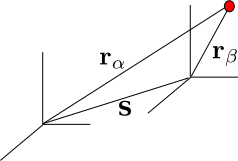
\includegraphics{noinercial}
  \caption{Sistema no inercial}
  \label{fig:noinercial}
\end{figure}

El movimiento de una partícula de masa $m$ visto desde el sistema inercial $\alpha$ y del sistema no inercial $\beta$ esta relacionado por
\begin{align*}
  \mathbf{r}_\alpha=\mathbf{r}_\beta+\mathbf{S}\,.
\end{align*}
derivando con respecto al tiempo obtenemos
\begin{align*}
   \mathbf{v}_\alpha=&\mathbf{v}_\beta+\mathbf{V}\nonumber\\
   \mathbf{a}_\alpha=&\mathbf{a}_\beta+\mathbf{A}\,,
\end{align*}
donde
\begin{align*}
  \mathbf{V}=&\dot{\mathbf{S}} &   \mathbf{A}=&\dot{\mathbf{V}}\,,  
\end{align*}
es la velocidad y aceleración del sistema no inercial con respecto al sistema inercial. 

El sistema inercial podemos aplicar la segunda ley de Newton
\begin{align*}
  \mathbf{F}=m \mathbf{a}_\alpha\,.
\end{align*}

Para un observador en el sistema no inercial la segunda Ley de Newton queda
\begin{align*}
  \mathbf{F}=&m \mathbf{a}_\beta+m\mathbf{A}\nonumber\\
  \mathbf{F}-m\mathbf{A}=&m \mathbf{a}_\beta\nonumber\\
  \mathbf{F}+\mathbf{F}_{\text{fict}}=&m \mathbf{a}_\beta\,.
\end{align*}
de modo que el observador en el sistema no inercial ve la aceleración de la partícula $\mathbf{a}_\beta$ como el resultado de la fuerza aplicada $\mathbf{F}$ y una fuerza ficticia
\begin{align*}
  \mathbf{F}_{\text{fict}}=-m\mathbf{A}\,.
\end{align*}
O de otro lado, un observador que requiera de fuerzas ficticias para describir el movimiento de una partícula, puede concluir que se encuentra en un sistema no inercial. Aunque normalmente se deben usar sistemas inerciales para hacer cálculo dinámicos, en algunos problemas es conveniente usar sistemas no inerciales.


\subsection{Mareas}
%Con este ejemplo se puede aclarar lo que significa campo gravitacional local
Las mareas son una evidencia de que la tierra se encuentra en un sistema noinercial. Sea $\boldsymbol{\mathcal{G}}(\mathbf{r}_{l}$ el campo gravitacional de la luna o el sol sobre el centro  de la tierra, con $\mathbf{r}_{l}$ la distancia desde el centro del cuerpo que ejerce el campo hasta el centro de la tierra. Un observador sobre la superficie de la tierra atribuye la marea a una fuerza ficticia $\mathbf{F}'$. De la ec.% 
tenemos
\begin{align}
  \mathbf{F}'=&\mathbf{F}+\mathbf{F}_{\text{fict}}\nonumber\\
  \mathbf{F}'=&m \boldsymbol{\mathcal{G}}(\mathbf{r})-m \boldsymbol{\mathcal{G}}(\mathbf{r}_l)
\end{align}

\subsection{Principio de equivalencia}



A partir de estos resultado podemos establecer el \emph{El principio de equivalencia}:
\begin{quote}
una fuerza ficticia $\mathbf{F}_{\text{fict}}=-m\mathbf{A}$ es indistinguible de la fuerza debido a un campo gravitacional uniforme (localmente)
\begin{align*}
  \boldsymbol{\mathcal{G}}=-\mathbf{A}\,.
\end{align*}
\end{quote}
En un campo gravitacional localmente constante $\boldsymbol{\mathcal{G}}$ una partícula de masa $m$ experimenta una fuerza
\begin{align*}
  \mathbf{F}=m\boldsymbol{\mathcal{G}}\,.
\end{align*}
La misma partícula en un sistema no inercial uniformemente acelerado con
\begin{align*}
  \mathbf{A}=-\boldsymbol{\mathcal{G}}
\end{align*}
sin presencia de campo gravitacional ni ninguna otra interacción, tenemos
\begin{align*}
   \mathbf{F}_{\text{fict}}=-m\mathbf{A}=m\boldsymbol{\mathcal{G}}\,,
\end{align*}
de donde
\begin{align*}
  \mathbf{A}=-\boldsymbol{\mathcal{G}}\,.
\end{align*}
No hay forma de distinguir localmente entre la aceleración gravitacional uniforme y un sistema de coordenadas con aceleración $\mathbf{A}=-\boldsymbol{\mathcal{G}}$. Localmente quiere decir que $\boldsymbol{\mathcal{G}}$ es constante en magnitud y dirección y que el sistema está confinado. Un observador no confinado si podría distinguir las dos situaciones. El carácter local de $\boldsymbol{\mathcal{G}}$ tiene que ver con el hecho de un campo gravitacional uniforme no puede extenderse a través de todo el espacio. 

Para ilustrar el principio de equivalencia considere un observador confinado dentro de un ascensor (sin ningún contacto con el exterior). En la primera situación el ascensor está cayendo libremente cerca de la superficie de la tierra. En la segunda situación el ascensor esta subiendo con una aceleración igual a la aceleración gravitacional. En ambos casos el observador se encuentra en un estado de ingravidez y ambos sistemas son indistinguible para el observador dentro del ascensor. Una situación similar ocurre en el interior de una nave espacial orbitando la tierra. A lo largo de la orbita el campo gravitacional es aproximadamente constante y la nave se encuentra en ``caída libre'' por lo que los astronautas están también en estado de ingravidez. En los entrenamientos de gravedad cero, se suele usar un avión el cual se deja caer desde una gran altura durante el tiempo que dura el estado de ingravidez. 




\begin{itemize}
\item[\textbf{Ejemplo:}] Un peso de masa $m$ cuelga de una cuerda en un vagón con aceleración constante de magnitud $A$. ¿Cómo puede un observador dentro del vagón aislado que se encuentra en un sistema no inercial? ¿Cual es ángulo estático de la cuerda con la horizontal y cual es la tensión?

\item[\textbf{Solución:}] 
Al encontrarse la posición de equilibrio del péndulo fuera de la vertical se necesita incluir un fuerza ficticia que implica que el vagón está en un estado de aceleración uniforme.

%De acuerdo a la figura
Las ecuaciones de movimiento en $x$ y $y$ desde un sistema inercial desde fuera del vagón:
\begin{align*}
  \text{En $x$:}&&T\sin\theta=&m A\nonumber\\
  \text{En $y$:}&&T\cos\theta-m g=&0\,,
\end{align*}
entonces
\begin{align}
  \label{eq:tencfic}
  T\cos\theta=&mg\nonumber\\
  T=&\frac{m g}{\cos\theta}\,,
\end{align}
y
\begin{align}
  \label{eq:tensfic}
  T\sin\theta=&m A\nonumber\\
  {m g}\frac{\sin\theta}{\cos\theta}=&mA\,,
\end{align}
de donde
\begin{align*}
  \tan\theta=\frac{A}{g}
\end{align*}
De la ecs.~\eqref{eq:tencfic} y \eqref{eq:tensfic}
\begin{align*}
  T^2(\cos^2\theta+\sin^2\theta)=m^2(A^2+g^2)\,,
\end{align*}
y
\begin{align*}
  T=m\sqrt{g^2+A^2}\,
\end{align*}

Las ecuaciones de movimiento desde el sistema no inercial con aceleración constante son
%ver figura
En $y$ es la misma que antes
\begin{align*}
  T\cos\theta-mg=&0\,,
\end{align*}
pero en $x$
\begin{align*}
    T\sin\theta-F_{\text{fict}}=0\,,
\end{align*}
Usando $F_{\text{fict}}=|\mathbf{F}_{\text{fict}}|=m A$, obtenemos
\begin{align*}
  T\sin\theta=m A\,,
\end{align*}
que corresponde a la ec.~\eqref{eq:tensfic}
\end{itemize}



%ejemplo pendulo oscilando en vagón


%%% Local Variables: 
%%% mode: latex
%%% TeX-master: "mecanica"
%%% End: 
